\subsection{pointer subterfuge}
\usetikzlibrary{calc}
\begin{frame}[fragile,label=pointerSub]{pointer subterfuge}
\lstset{
    language=C,
    style=small,
    moredelim={**[is][\btHL<2|handout:0>]{~2~}{~end~}},
    morekeywords={size_t},
}
\begin{lstlisting}
void f2b(void *arg, size_t len) {
    char buffer[100];
    long val = ...; /* assume on stack */
    long *ptr = ...; /* assume on stack */
    memcpy(buff, arg, len); /* overwrite ptr? */
    ~2~*ptr = val~end~; /* arbitrary memory write! */
}
\end{lstlisting}
\imagecredit{adapted from Pincus and Baker, Figure 2}
% FIXME: stack picture
\end{frame}





\section{arbitrary writes}

\begin{frame}<1-3>[label=arbWrite]{arbitrary memory write}
    \begin{itemize}
    \item bunch of scenarios that lead to \myemph{single arbitrary memory write}
        \begin{itemize}
        \item format exploits are one, but we'll find more!!
        \end{itemize}
    \item typical result: arbitrary code execution
    \item how?
    \vspace{.5cm}
    \item<2-> \myemph<3>{overwrite existing machine code (insert jump?)}
        \begin{itemize}
        \item problem: usually not writable
        \end{itemize}
    \item<2-> \myemph<4>{overwrite return address directly}
        \begin{itemize}
        \item observation: don't care about stack canaries --- skip them
        \end{itemize}
    \item<2-> \myemph<5>{overwrite other function pointer?}
    \item<2-> \myemph<6>{overwrite another data pointer --- copy more?}
    \end{itemize}
\end{frame}


\againframe<3>{arbWrite}

\subsection{example: return address overwrite}
\againframe<4>{arbWrite}
\usetikzlibrary{arrows.meta}
\begin{frame}[fragile,label=skipCanary]{skipping the canary}
\begin{tikzpicture}
% FIXME:
\tikzset{
    stackBox/.style={very thick},
    onStack/.style={thick},
}
\begin{scope}[xscale=1.2]
\draw[stackBox] (0, 0) rectangle (10, -6);
\draw[thick,-Latex] (10.25,-5) -- (10.25, -1) node [midway, below, sloped] {increasing addresses};
\node[at={(5, 0.1)},anchor=south] { highest address (stack started here)};
\node[at={(5, -6.1)},anchor=north] { lowest address (stack grows here)};

\draw[onStack] (0, -.25) rectangle (10, -1.25) node[midway,align=center,font=\small] (stackAddr)
     {return address for {\tt f2b} };
\draw[onStack,fill=red!20] (0, -1.25) rectangle (10, -2.25) node[midway,align=center,font=\small] (canaryAddr)
     {stack canary};
\draw[onStack,fill=green!20] (0, -2.25) rectangle (10, -2.75) node[midway,align=center,font=\small] (ptr) {ptr (8 bytes)};
\draw[onStack,fill=green!20] (0, -2.75) rectangle (10, -3.25) node[midway,align=center,font=\small] (val) {val (8 bytes)};
\draw[onStack,fill=blue!20] (0, -3.25) rectangle (10, -5.25) node[midway,align=center,font=\small] {buffer (100 bytes)};

\draw[onStack] (0, -5.25) rectangle (10, -6) node[midway,align=center,font=\small] {return address for {\tt scanf}};

\begin{visibleenv}<2->
\draw[-Latex,orange,ultra thick] ([xshift=1cm]ptr.east) -- ++(2cm,0cm) |- (stackAddr.east);
\draw[-Latex,orange,ultra thick,dashed] ([xshift=1cm]val.east) -- ++(2cm,0cm) |- (0.25, -5);
\end{visibleenv}

\begin{visibleenv}<3>
\draw[-Latex,red,ultra thick] ([yshift=2.5mm]stackAddr.south east) -- ++(.25cm,0cm) |- (0.25, -5);
\node[anchor=south west,red] at (0.25, -4.75) {
    machine code for the attacker to run
};
\end{visibleenv}
\end{scope}
\end{tikzpicture}
\end{frame}


\subsection{exercise}
\begin{frame}[fragile]{exercise (1)}
\begin{tikzpicture}
\node (left) {
\begin{lstlisting}[language=C,style=size9]
void vulnerable() {
    int *array;
    char buffer[100];
    if (!Allocate(&array))
        abort();
    gets(buffer);
    array[0] = atoi(buffer);
    ...
}
\end{lstlisting}
};
\node[anchor=north west] at ([xshift=4cm]left.north east) {
\begin{lstlisting}[language=myasm,style=size9]
vulnerable:
    pushq %rbp
    pushq %rbx
    subq  $136, %rsp
    movq  %fs:40, %rax
    movq  %rax, 120(%rsp)
    xorl  %eax, %eax
    leaq  104(%rsp), %rdi
    call  Allocate
    testl %eax, %eax
    je    call_abort
    movq  %rsp, %rdi
    call  gets
    movq  104(%rsp), %rbp
    movl  $10, %edx
    movl  $0, %esi
    movq  %rsp, %rdi
    call  strtol
    movl  %eax, 0(%rbp)
    ...
\end{lstlisting}
};
\node[align=left,draw,very thick,anchor=north west] at (left.south west) {
If return address is at 0x12345, \\
where/how to place 0x12345 in input?  \\
{\fontsize{9}{10}\selectfont\begin{tabular}{l}
A. beginning, as ASCII base-10 number \\
B. beginning, as ASCII base-16 number \\
C. 100 bytes into buffer, as bytes \\
D. 104 bytes into buffer, as bytes \\
E. 120 bytes into buffer, as bytes \\
F. 136 bytes into buffer, as bytes \\
G. none of these \\
\end{tabular}}
};
\end{tikzpicture}
\end{frame}

\begin{frame}[fragile]{exercise (2)}
\begin{tikzpicture}
\node (left) {
\begin{lstlisting}[language=C,style=size9]
void vulnerable() {
    int *array;
    char buffer[100];
    if (!Allocate(&array))
        abort();
    gets(buffer);
    array[0] = atoi(buffer);
    ...
}
\end{lstlisting}
};
\node[anchor=north west] at ([xshift=4cm]left.north east) {
\begin{lstlisting}[language=myasm,style=size9]
vulnerable:
    pushq %rbp
    pushq %rbx
    subq  $136, %rsp
    movq  %fs:40, %rax
    movq  %rax, 120(%rsp)
    xorl  %eax, %eax
    leaq  104(%rsp), %rdi
    call  Allocate
    testl %eax, %eax
    je    call_abort
    movq  %rsp, %rdi
    call  gets
    movq  104(%rsp), %rbp
    movl  $10, %edx
    movl  $0, %esi
    movq  %rsp, %rdi
    call  strtol
    movl  %eax, 0(%rbp)
    ...
\end{lstlisting}
};
\node[align=left,draw,very thick,anchor=north west] at (left.south west) {
If we want to overwrite ret. addr. with 0x5678, \\
where/how to place 0x5678 in input? \\
{\fontsize{9}{10}\selectfont\begin{tabular}{l}
A. beginning, as ASCII base-10 number \\
B. beginning, as ASCII base-16 number \\
C. 100 bytes into buffer, as bytes \\
D. 104 bytes into buffer, as bytes \\
E. 120 bytes into buffer, as bytes \\
F. 136 bytes into buffer, as bytes \\
G. none of these \\
\end{tabular}}
};
\end{tikzpicture}
\end{frame}


\subsubsection{careful stack layout?}
\begin{frame}{laying out stack to avoid subterfuge (1)}
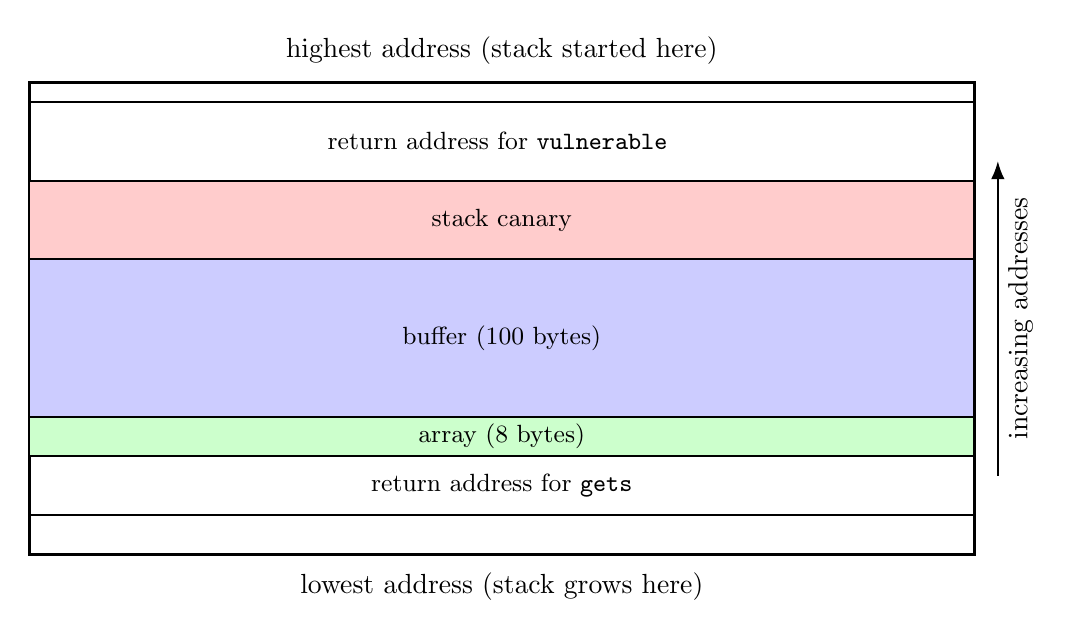
\begin{tikzpicture}
% FIXME:
\tikzset{
    stackBox/.style={very thick},
    onStack/.style={thick},
}
\begin{scope}[xscale=1.2]
\draw[stackBox] (0, 0) rectangle (10, -6);
\draw[thick,-Latex] (10.25,-5) -- (10.25, -1) node [midway, below, sloped] {increasing addresses};
\node[at={(5, 0.1)},anchor=south] { highest address (stack started here)};
\node[at={(5, -6.1)},anchor=north] { lowest address (stack grows here)};

\draw[onStack] (0, -.25) rectangle (10, -1.25) node[midway,align=center,font=\small] (stackAddr)
     {return address for {\tt vulnerable} };
\draw[onStack,fill=red!20] (0, -1.25) rectangle (10, -2.25) node[midway,align=center,font=\small] (canaryAddr)
     {stack canary};
\draw[onStack,fill=blue!20] (0, -2.25) rectangle (10, -4.25) node[midway,align=center,font=\small] {buffer (100 bytes)};

\draw[onStack,fill=green!20] (0, -4.25) rectangle (10, -4.75) node[midway,align=center,font=\small] (ptr) {array (8 bytes)};
\draw[onStack] (0, -4.75) rectangle (10, -5.5) node[midway,align=center,font=\small] {return address for {\tt gets}};

\end{scope}
\end{tikzpicture}
\end{frame}

\begin{frame}{laying out stack to avoid subterfuge (2)}
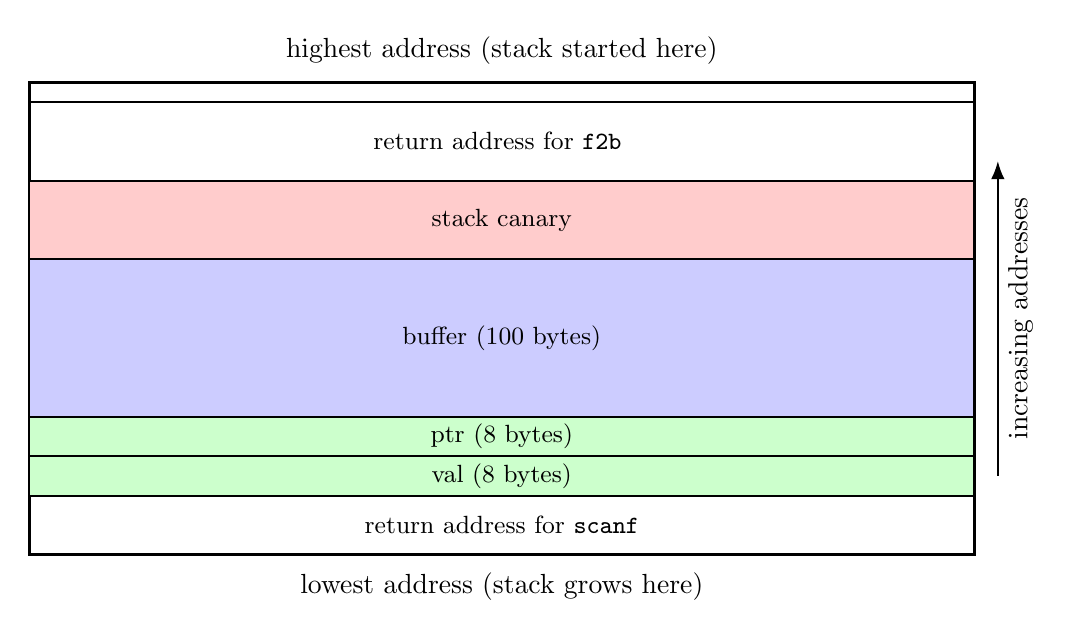
\begin{tikzpicture}
% FIXME:
\tikzset{
    stackBox/.style={very thick},
    onStack/.style={thick},
}
\begin{scope}[xscale=1.2]
\draw[stackBox] (0, 0) rectangle (10, -6);
\draw[thick,-Latex] (10.25,-5) -- (10.25, -1) node [midway, below, sloped] {increasing addresses};
\node[at={(5, 0.1)},anchor=south] { highest address (stack started here)};
\node[at={(5, -6.1)},anchor=north] { lowest address (stack grows here)};

\draw[onStack] (0, -.25) rectangle (10, -1.25) node[midway,align=center,font=\small] (stackAddr)
     {return address for {\tt f2b} };
\draw[onStack,fill=red!20] (0, -1.25) rectangle (10, -2.25) node[midway,align=center,font=\small] (canaryAddr)
     {stack canary};
\draw[onStack,fill=blue!20] (0, -2.25) rectangle (10, -4.25) node[midway,align=center,font=\small] {buffer (100 bytes)};

\draw[onStack,fill=green!20] (0, -4.25) rectangle (10, -4.75) node[midway,align=center,font=\small] (ptr) {ptr (8 bytes)};
\draw[onStack,fill=green!20] (0, -4.75) rectangle (10, -5.25) node[midway,align=center,font=\small] (val) {val (8 bytes)};
\draw[onStack] (0, -5.25) rectangle (10, -6) node[midway,align=center,font=\small] {return address for {\tt scanf}};

\end{scope}
\end{tikzpicture}
\end{frame}



\subsubsection{structs containing pointers}
\usetikzlibrary{arrows.meta}
\begin{frame}[fragile,label=structSubter]{other subterfuge cases (1)}
\begin{lstlisting}[language=C,style=small]
struct Command {
  CommandType type;
  int values[MAX_VALUES];
  int *active_value;
  ...
};
\end{lstlisting}
\begin{tikzpicture}[overlay,remember picture]
% FIXME:
\tikzset{
    stackBox/.style={very thick},
    onStack/.style={thick},
}
\coordinate (my anchor) at ([xshift=-9cm,yshift=-2cm]current page.north east);
\begin{scope}[shift={(my anchor)},xscale=0.8]
\draw[stackBox] (0, 0) rectangle (10, -6);
\draw[thick,-Latex] (10.25,-5) -- (10.25, -1) node [midway, below, sloped] {increasing addresses};
\node[at={(5, 0.1)},anchor=south] { highest address };
\node[at={(5, -6.1)},anchor=north] { lowest address };

\draw[onStack] (0, -.25) rectangle (10, -2.25) node[midway,align=center,font=\small] (stackAddr)
     {more struct fields};
\draw[onStack,fill=green!20] (0, -2.25) rectangle (10, -2.75) node[midway,align=center,font=\small] (ptr) {active\_value};
\draw[onStack,fill=blue!20] (0, -2.75) rectangle (10, -5.25) node[midway,align=center,font=\small] {values};
\draw[onStack,fill=yellow!20] (0, -5.25) rectangle (10, -5.75) node[midway,align=center,font=\small] {type};
\end{scope}
\end{tikzpicture}
\end{frame}

\begin{frame}[fragile,label=globalSubter]{other subterfuge cases (2)}
\begin{lstlisting}[language=C,style=small]
Command *current_command;
char input_buffer[4096];

void run_next_command() {
  if (!current_command) {
    current_command =
        getNext();
  }
  current_command-> ...
  ...
}
\end{lstlisting}
\begin{tikzpicture}[overlay,remember picture]
% FIXME:
\tikzset{
    stackBox/.style={very thick},
    onStack/.style={thick},
}
\coordinate (my anchor) at ([xshift=-9cm,yshift=-2cm]current page.north east);
\begin{scope}[shift={(my anchor)},xscale=0.8]
\draw[stackBox] (0, 0) rectangle (10, -6);
\draw[thick,-Latex] (10.25,-5) -- (10.25, -1) node [midway, below, sloped] {increasing addresses};
\node[at={(5, 0.1)},anchor=south] { highest address };
\node[at={(5, -6.1)},anchor=north] { lowest address };

\draw[onStack] (0, -.25) rectangle (10, -2.25) node[midway,align=center,font=\small] (stackAddr)
     {more globals};
\draw[onStack,fill=green!20] (0, -2.25) rectangle (10, -2.75) node[midway,align=center,font=\small] (ptr) {current\_command};
\draw[onStack,fill=blue!20] (0, -2.75) rectangle (10, -5.25) node[midway,align=center,font=\small] {input\_buffer};
\draw[onStack] (0, -5.25) rectangle (10, -5.75) node[midway,align=center,font=\small] {more globals};
\end{scope}
\end{tikzpicture}
\end{frame}


\section{beyond stack smashing}
\begin{frame}{beyond return addresses}
    \begin{itemize}
    \item pointer subterfuge let us overwrite anything
    \item my example: showed return address
    \item but return address is tricky to locate exactly
    \item but there are \myemph{easier options!}
    \end{itemize}
\end{frame}




\section{write targets, continued}
\subsection{example: GOT overwrite}
\againframe<5>{arbWrite}

\begin{frame}[fragile,label=gotOverwrite]{attacking the GOT}
\begin{tikzpicture}
% FIXME:
\tikzset{
    stackBox/.style={very thick},
    onStack/.style={thick},
}
\draw[stackBox] (0, 0) rectangle (10, -6);
\draw[thick,-Latex] (10.25,-5) -- (10.25, -1) node [midway, below, sloped] {increasing addresses};
\node[at={(5, 0.1)},anchor=south] { highest address (stack started here)};
\node[at={(5, -6.1)},anchor=north] { lowest address (stack grows here)};

\draw[onStack] (0, -.25) rectangle (10, -1.25) node[midway,align=center,font=\small] (stackAddr)
     {return address for {\tt f2b} };
\draw[onStack,fill=red!20] (0, -1.25) rectangle (10, -2.25) node[midway,align=center,font=\small] (canaryAddr)
     {stack canary};
\draw[onStack,fill=green!20] (0, -2.25) rectangle (10, -2.75) node[midway,align=center,font=\small] (ptr) {ptr (8 bytes)};
\draw[onStack,fill=green!20] (0, -2.75) rectangle (10, -3.25) node[midway,align=center,font=\small] (val) {val (8 bytes)};
\draw[onStack,fill=blue!20] (0, -3.25) rectangle (10, -5.25) node[midway,align=center,font=\small] {buffer (100 bytes)};

\draw[onStack] (0, -5.25) rectangle (10, -6) node[midway,align=center,font=\small] {return address for {\tt scanf}};

\node[anchor=south] at (13.5, -1) { global offset table };
\draw[stackBox] (11.5, -1) rectangle (15.25, -1.5) node[midway,font=\small] (printfEntry) {GOT entry: printf };
\draw[stackBox] (11.5, -1.5) rectangle (15.25, -2) node[midway,font=\small] {GOT entry: fopen };
\draw[stackBox] (11.5, -2) rectangle (15.25, -2.5) node[midway,font=\small] {GOT entry: exit };

\begin{visibleenv}<2->
\draw[-Latex,orange,ultra thick] ([xshift=1cm]ptr.east) -- ++(2cm,0cm) |- (printfEntry.west);
\draw[-Latex,orange,ultra thick,dashed] ([xshift=1cm]val.east) -- ++(2cm,0cm) |- (0.25, -5);
\end{visibleenv}

\begin{visibleenv}<3>
\draw[-Latex,red,ultra thick] ([yshift=2.5mm]printfEntry.south east) -- ++(.25cm,0cm) |- (0.25, -5);
\node[anchor=south west,red,inner sep=0.1mm] at (0.25, -4.75) {
    machine code for the attacker to run
};
\end{visibleenv}
\end{tikzpicture}
\end{frame}



\subsection{C++ inheritence}
\againframe<5>{arbWrite}
\usetikzlibrary{arrows.meta,matrix}

\begin{frame}[fragile,label=CPPVirt]{C++ inheritence}
\lstset{
    language=C++,style=smaller,
}
\begin{lstlisting}
class InputStream {
public:
    virtual int get() = 0;
    // Java: abstract int get();
    ...
};
class SeekableInputStream : public InputStream {
public:
    virtual void seek(int offset) = 0;
    virtual int tell() = 0;
};
class FileInputStream : public InputStream {
public:
    int get();
    void seek(int offset);
    int tell();
    ...
};
\end{lstlisting}
\end{frame}

\begin{frame}<1>[label=inheritMemLay]{C++ inheritence: memory layout}
\begin{tikzpicture}
    \tikzset{
        vt/.style={fill=blue!30},
    }
    \matrix[tight matrix,nodes={text width=3.8cm,text depth=.1ex,font=\small\tt},
            label={north:InputStream},anchor=north west] (inputStream)  at (0, 0) {
        |[vt]| vtable pointer \\
    };
    \matrix[tight matrix,nodes={text width=3.8cm,text depth=.1ex,font=\small\tt},
            label={north:SeekableInputStream},anchor=north west] (seekableStream) at (4.5, 0) {
        |[vt]| vtable pointer \\
    };
    \matrix[tight matrix,nodes={text width=6cm,text depth=.1ex,font=\small\tt},
            label={north:FileInputStream},anchor=north west] (fileStream) at (9, 0) {
        |[vt]| vtable pointer \\
        file\_pointer \\
    };
    \matrix[tight matrix,nodes={text width=3.8cm,text depth=.1ex,font=\small\tt},anchor=north west] (isVT) at (0, -2) {
        \tt slot for get\\
    };
    \matrix[tight matrix,nodes={text width=3.8cm,text depth=.1ex,font=\small\tt},anchor=north west] (seekVT) at (4.5, -2){
        \tt slot for get \\
        \tt slot for seek \\
        \tt slot for tell \\
    };
    \matrix[tight matrix,nodes={text width=6cm,text depth=.1ex,font=\small\tt},anchor=north west] (fileVT) at (9, -2){
        FileInputStream::get \\
        FileinputStream::seek \\
        FileInputStream::tell \\
    };
    \draw[thick,-Latex] (inputStream-1-1.east) -- ++(.35cm,0cm) |- (isVT-1-1.east);
    \draw[thick,-Latex] (seekableStream-1-1.east) -- ++(.35cm,0cm) |- (seekVT-1-1.east);
    \draw[thick,-Latex] (fileStream-1-1.east) -- ++(.35cm,0cm) |- (fileVT-1-1.east);
\end{tikzpicture}
\end{frame}

\begin{frame}[fragile,label=CPPImpl]{C++ implementation (pseudo-code)}
\lstset{
    language=C,style=smaller,
}
\begin{lstlisting}
struct InputStream_vtable {
    int (*get)(InputStream* this);
};

struct InputStream {
    InputStream_vtable *vtable;
};

...

    InputStream *s = ...;
    int c = (s->vtable->get)(s);
\end{lstlisting}
\end{frame}

\begin{frame}[fragile,label=CPPImplB]{C++ implementation (pseudo-code)}
\lstset{
    language=C,style=smaller,
}
\begin{lstlisting}
struct SeekableInputStream_vtable {
    struct InputStream_vtable as_InputStream;
    void (*seek)(SeekableInputStream* this, int offset);
    int (*tell)(SeekableInputStream* this);
};

struct FileInputStream {
    SeekableInputStream_vtable *vtable;
    FILE *file_pointer;
};

...

    FileInputStream file_in = { the_FileInputStream_vtable,  ... };
    InputStream *s = (InputStream*) &file_in;
\end{lstlisting}
\end{frame}

\begin{frame}[fragile,label=CPPImplC]{C++ implementation (pseudo-code)}
\lstset{
    language=C,style=smaller,
}
\begin{lstlisting}
SeekableInputStream_vtable the_FileInputStream_vtable = {
    &FileInputStream_get,
    &FileInputStream_seek,
    &FileInputStream_tell,
};

...

    FileInputStream file_in = { the_FileInputStream_vtable,  ... };
    InputStream *s = (InputStream*) &file_in;
\end{lstlisting}
\end{frame}




\subsection{options for attacking function pointer tables}
    % FIXME: find another function pointer in memory

\begin{frame}{attacking function pointer tables}
% FIXME: picture
\begin{itemize}
\item option 1: overwrite table entry directly  
    \begin{itemize}
    \item required/easy for Global Offset Table --- fixed location
    \item usually not possible for VTables --- read-only memory
    \end{itemize}
\item option 2: create table in buffer (big list of pointers to shellcode), point to buffer
    \begin{itemize}
    \item useful when table pointer next to buffer
    \item (e.g. C++ object on stack next to buffer)
    \end{itemize}
\item option 3: find suitable pointer elsewhere
    \begin{itemize}
    \item e.g. point to wrong part of vtable to run different function
    \end{itemize}
\end{itemize}
\end{frame}




\subsection{vtable overwrite exercise}
\usetikzlibrary{arrows.meta,matrix}
\begin{frame}[fragile,label=vtExer]{exercise}
\vspace{-.25cm}
\begin{tikzpicture}
    \tikzset{
        vt/.style={fill=blue!30},
    }
    \matrix[tight matrix,nodes={text width=3.8cm,text depth=.1ex,font=\small\tt},
            label={north:objArray},anchor=north west] (vulnClass)  at (0, 0) {
        |[vt]| vtable pointer \\
        |[minimum height=1cm]| buffer\\
        |[vt]| vtable pointer \\
        |[minimum height=1cm]| \ldots \\
    };
    \matrix[tight matrix,nodes={text width=3.8cm,text depth=.1ex,font=\small\tt},anchor=north west] (isVT) at (0, -3) {
        \tt slot for foo\\
        \tt slot for bar\\
    };
    \draw[thick,-Latex] (vulnClass-1-1.east) -- ++(.45cm,0cm) |- (isVT-1-1.east);
    \draw[thick,-Latex] (vulnClass-3-1.east) -- ++(.35cm,0cm) |- (isVT-1-1.east);
    \node[anchor=north west] at (5, 0) {
\begin{lstlisting}[language=C++,style=smaller]
class VulnerableClass {
public:
    char buffer[100];
    virtual void foo();
    virtual void bar();
};
VulnerableClass objArray[10];
\end{lstlisting}
};
\end{tikzpicture}
\begin{itemize}
\item if we can overflow \texttt{objArray[0].buffer} to change array[1]'s vtable pointer and know array[1].foo() will be called; finish the plan:
\end{itemize}
\small \begin{tabular}{ll}
buffer[0]: \rule{2cm}{.1mm} \hspace{1cm} & A. shellcode \\
buffer[50]: \rule{2cm}{.1mm} \hspace{1cm} & B. address of buffer[0]\\
array[1]'s vtable pointer: \rule{2cm}{.1mm} \hspace{1cm} & C. address of buffer[50] \\
~ & D. address of original vtable \\
~ & E. address of objArray[0]'s vtable \\
~ & E. address of objArray[1]'s vtable pointer \\
\end{tabular}
\end{frame}





\section{one write into another}
\againframe<6>{arbWrite}


\section{arc injection}
\begin{frame}{so far overwrites}
    \begin{itemize}
    \item once we found a way to overwrite function pointer\\
          easiest solution seems to be: direct to our code
    \item \ldots but alterante places to direct it to
    \end{itemize}
\end{frame}

\usetikzlibrary{arrows.meta}

\begin{frame}[fragile,label=returnToSomewhere]{return-to-somewhere}
\begin{tikzpicture}
% FIXME:
\tikzset{
    stackBox/.style={very thick},
    onStack/.style={thick},
}
\begin{scope}[xscale=0.75]
\draw[stackBox] (0, 0) rectangle (10, -6);
\draw[thick,-Latex] (10.25,-5) -- (10.25, -1) node [midway, below, sloped] {increasing addresses};
\node[at={(5, 0.1)},anchor=south] { highest address (stack started here)};
\node[at={(5, -6.1)},anchor=north] { lowest address (stack grows here)};

\draw[onStack] (0, -.25) rectangle (10, -1.25) node[midway,align=center,font=\small] (stackAddr)
     {return address for {\tt vulnerable}: \\ address of {\tt do\_useful\_stuff}};
\draw[onStack,fill=black!20] (0, -1.25) rectangle (10, -2.25) node[midway,align=center,font=\small] {unused space (20 bytes)};
\draw[onStack,fill=blue!20] (0, -2.25) rectangle (10, -5.25) node[midway,align=center,font=\small] {buffer (100 bytes)};

\draw[onStack] (0, -5.25) rectangle (10, -6) node[midway,align=center,font=\small] {return address for {\tt scanf}};

\draw[onStack,fill=red!20,opacity=0.9] (0, -5.25) rectangle (10, -1.25) node[midway,align=center,font=\small,text=red!50!black] {unused junk};

\draw[-Latex,red,ultra thick,dashed] ([yshift=2.5mm]stackAddr.south east) -- ++(.25cm,0cm) |-
    (11, -4.25) node[align=left,right,font=\small] { {\tt do\_useful\_stuff} \\ (already in program) };

\begin{visibleenv}<2>
\fill[white,opacity=0.5, overlay] (-1,-2) rectangle (18, -8);
\end{visibleenv}
\end{scope}
\end{tikzpicture}
\begin{tikzpicture}[overlay,remember picture]
\begin{visibleenv}<2>
\node[fill=white,draw,ultra thick,align=center,anchor=center] at (current page.center) {
    code is \myemph{already in program}??? \\
    how often does this happen??? \\
    \ldots turns out ``\myemph{usually}'' --- more later in semester
};
\end{visibleenv}
\end{tikzpicture}
\end{frame}

\begin{frame}[fragile,label=systemFunc]{example: system()}
\begin{lstlisting}[language={}]
NAME
       system - execute a shell command

SYNOPSIS
       #include <stdlib.h>

       int system(const char *command);
\end{lstlisting}
\begin{itemize}
\item part of C standard library
\item in any program that dynamically links to libc
\item challenge: need to hope argument register (rdi) set usefully
\end{itemize}
\end{frame}

\begin{frame}[fragile,label=locateSystem]{locating system() Linux}
\begin{lstlisting}[language={},style=script,
moredelim={**[is][\btHL<1>]{~1~}{~end~}},
]
$ ldd /bin/ls
        linux-vdso.so.1 (0x00002aaaaaade000)
        libselinux.so.1 => /lib/x86_64-linux-gnu/libselinux.so.1 (0x00002aaaaab3a000)
        libc.so.6 => /lib/x86_64-linux-gnu/libc.so.6 (~1~0x00002aaaaab65000~end~)
        libpcre2-8.so.0 => /usr/lib/x86_64-linux-gnu/libpcre2-8.so.0 (0x00002aaaaad57000)
        libdl.so.2 => /lib/x86_64-linux-gnu/libdl.so.2 (0x00002aaaaade7000)
        /lib64/ld-linux-x86-64.so.2 (0x00002aaaaaaab000)
        libpthread.so.0 => /lib/x86_64-linux-gnu/libpthread.so.0 (0x00002aaaaaded000)
$ objdump --dynamic-syms /lib/x86_64-linux-gnu/libc.so.6 | grep system
0000000000156a80 g    DF .text  0000000000000067  GLIBC_2.2.5 svcerr_systemerr
0000000000055410 g    DF .text  000000000000002d  GLIBC_PRIVATE __libc_system
~1~0000000000055410~end~  w   DF .text  000000000000002d  GLIBC_2.2.5 system
\end{lstlisting}
\begin{itemize}
\item if address randomization disabled: \\
address should be 0x00002aaaaab650 + 0x55410
\vspace{.5cm}
\item \texttt{ldd} --- ``what libraries does this load and where?''
    \begin{itemize}
    \item similar tools for other OSes
    \end{itemize}
\end{itemize}
\end{frame}


\section{case study: NTP exploit}
\usetikzlibrary{arrows.meta,patterns}
\begin{frame}[fragile,label=ntpStudyIntro]{case study (simplified)}
    \begin{itemize}
    \item bug in NTPd (Network Time Protocol Daemon)
    \item via Stephen R\"ottger, ``Finding and exploiting ntpd vulnerabilities''
        \begin{itemize}
        \item \url{https://googleprojectzero.blogspot.com/2015/01/finding-and-exploiting-ntpd.html}
        \end{itemize}
    \end{itemize}
\lstset{
    language=C,
    style=small,
    moredelim={**[is][\btHL<1|handout:0>]{~1~}{~end~}},
    moredelim={**[is][\btHL<2|handout:0>]{~2~}{~end~}},
}
\begin{lstlisting}
static void
ctl_putdata(
  const char *dp,
  unsigned int dlen,
  int bin   /* set to 1 when data is binary */
  ) {
    ...
    ~1~memmove((char *)datapt, dp, (unsigned)dlen);~end~
    datapt += dlen;
    datalinelen += dlen;
}
\end{lstlisting}
\end{frame}

\begin{frame}<1>[fragile,label=target]{the target}
\lstset{
    language=C,
    style=small,
    moredelim={**[is][\btHL<1|handout:0>]{~1~}{~end~}},
    moredelim={**[is][\btHL<2|handout:0>]{~2~}{~end~}},
}
\begin{lstlisting}
    memmove((char *)~1~datapt~end~, dp, (unsigned)dlen);
\end{lstlisting}
\begin{tikzpicture}
\tikzset{box/.style={thick}}
\draw[box,fill=blue!20] (0, 0) rectangle (10, -0.5) node[midway] (datapt) {datapt (global variable)};
\draw[box,fill=green!20] (0, -0.5) rectangle (10, -1.5) node[midway] {(other global variables)};
\draw[box,fill=red!20] (0, -1.5) rectangle (10, -2.5) node[midway] (buffer) {buffer (global array)};
\begin{visibleenv}<1-2>
    \draw[very thick,violet!70!black,-Latex] (datapt.west) -- ++(-.5cm,0cm) -| (0.5, -1.75);
\end{visibleenv}
\begin{visibleenv}<2->
    \draw[box,fill=orange!20] (11, -1) rectangle (15, -1.5) node[midway] (strlen) {strlen GOT entry};
\end{visibleenv}
\begin{visibleenv}<3->
    \fill[pattern=north west lines,pattern color=red,opacity=0.4] (0, -2.5) rectangle (10, 0);
    \draw[-Latex,very thick,dashed,red] (datapt) -| ([xshift=-0.5cm]strlen.west) -- (strlen.west);
\end{visibleenv}
\begin{visibleenv}<4->
    \draw[box,fill=violet!20] (11, -3) rectangle (15, -3.5) node[midway] (system) {{\tt system()} stub};
    \fill[pattern=north west lines,pattern color=red,opacity=0.4] (11, -1) rectangle (15, -1.5);
    \draw[-Latex,very thick,dashed,red] (strlen.south) -- (system.north);
\end{visibleenv}
\end{tikzpicture}
\end{frame}

\begin{frame}[fragile,label=moreContext]{more context}
\lstset{
    language=C,
    moredelim={**[is][\btHL<1|handout:0>]{~1~}{~end~}},
    moredelim={**[is][\btHL<2|handout:0>]{~2~}{~end~}},
}
\begin{lstlisting}
    memmove((char *)~1~datapt~end~, dp, (unsigned)dlen);
    ...
    ...
    strlen(some_user_supplied_string)
    /* calls strlen@plt
       looks up global offset table entry! */
\end{lstlisting}
\end{frame}

\againframe<2>{target}

\begin{frame}{overall exploit}
    \begin{itemize}
    \item overwrite {\tt datapt} to point to strlen GOT entry
    \item overwrite value of strlen GOT entry
    \item example target: {\tt system} function
            \begin{itemize}
                \item executes command-line command specified by argument
            \end{itemize}
    \item supply string to provide argument to ``{\tt strlen}''
    \end{itemize}
\end{frame}

\againframe<3->{target}

\begin{frame}{overall exploit: reality}
    \begin{itemize}
    \item real exploit was more complicated
    \item needed to defeat more mitigations
    \item needed to deal with not being able to write {\tt \textbackslash 0}
    \item actually tricky to send things that trigger buffer write
        \begin{itemize}
        \item (meant to be local-only)
        \end{itemize}
    \end{itemize}
\end{frame}



\subsection{subterfuge exercise}
\begin{frame}[fragile,label=subterExer]{subterfuge exercise}
\begin{lstlisting}[language=C++,style=script]
struct Student {
    char email[128];
    struct Assignment *assignments[16];
    ...
};
struct Assignment {
    char submission_file[128];
    char regrade_request[1024];
    ...
};
void SetEmail(Student *s, char *new_email) { strcpy(s->email, new_email); }
void AddRegradeRequest(Student *s, int index, char *request) {
    strcpy(s->assignments[index]->regrade_request, request);
}
void vulnerable(char *STRING1, char *STRING2) {
    SetEmail(s, STRING1); AddRegradeRequest(s, 0, STRING2);
}
\end{lstlisting}
\begin{itemize}
\item exercise: to set \texttt{0x1020304050} to \texttt{0xAABBCCDD}, what should STRING1, STRING2 be?
    \begin{itemize}
    \item (assume 64-bit pointers, no padding in structs, little-endian)
    \end{itemize}
\end{itemize}
\end{frame}

